\section{Experimental Results}
\label{sec:ExpResults}

\subsection{Resource Utilization}
\label{sec:resource_utilization}

\begin{table}[t]
\centering
\caption{Post place-and-route resource utilization on Alveo U280.}
\label{tab:resource_annotated}
\resizebox{\columnwidth}{!}{
\begin{tabular}{l l r r r r r}
\toprule
Algorithm & Config & FF & LUTs & DSPs & BRAMs & Freq \\
\midrule
MiniRocket & Fused 1CU & 94,283 & 57,090 & 0 & 185 & 300 MHz \\
MiniRocket & Fused 2CU & 188,566 & 114,180 & 0 & 370 & 300 MHz \\
MiniRocket & Fused 3CU & 159,086 & 92,703 & 1,264 & 428 & 269 MHz \\
MiniRocket & DP-Reuse 1CU & 153,327 & 135,634 & 2 & 1,320 & 300 MHz \\
\addlinespace
HYDRA & v2\_fixed 1CU & 58,537 & 41,746 & 1,355 & 86 & 300 MHz \\
HYDRA & Dataflow 1CU & 20,823 & 15,866 & 55 & 115 & 405 MHz \\
\bottomrule
\end{tabular}}
\end{table}


Table \ref{tab:resource_annotated} reports post place-and-route resource utilization on the Alveo U280. All single-node designs achieve 300\,MHz; the 3-CU MiniRocket variant is auto-throttled to 269\,MHz due to SLR crossing penalties.

MiniRocket's fused CONV+PPV kernel achieves zero DSP utilization by exploiting the ternary weight structure ($\{-1, +2\}$) through the bFP multiplier (Eq. \ref{eq:bFP}). Hydra's v2\_fixed variant uses 1,355 DSPs because its learned random kernels require standard floating-point multiplication, implemented via ap\_fixed$\langle$32,16$\rangle$ arithmetic.

\subsection{Throughput, Latency, and Accuracy}
\label{sec:single_node_results}

\begin{table}[t]
\centering
\caption{Throughput (inferences/sec) and classification accuracy (\%). Baseline = single-threaded C++ \texttt{-O3 -march=native} on the same kernel source compiled natively (HLS pragmas no-op); Speedup = FPGA 3CU / C++ baseline.}
\label{tab:throughput}
\resizebox{\columnwidth}{!}{
\begin{tabular}{l l r r r r r r r}
\toprule
Algorithm & Dataset & Len & C++ Base & FPGA 1CU & FPGA 3CU & Speedup & Ref Acc & FPGA Acc \\
\midrule
MiniRocket & InsectSound & 600 & 289 & 1,967 & 5,012 & 17.3$\times$ & 78.84 & 74.12 \\
MiniRocket & MosquitoSound & 3,750 & 48 & 937 & 2,820 & 58.7$\times$ & 87.59 & 87.88 \\
MiniRocket & FruitFlies & 5,000 & 258 & 742 & 2,191 & 8.5$\times$ & 96.98 & 95.82 \\
\addlinespace
HYDRA & InsectSound & 600 & 1,372 & 6,326 & 10,573 & 7.7$\times$ & 69.41 & 69.41 \\
HYDRA & MosquitoSound & 3,750 & 326 & 1,937 & 3,516 & 10.8$\times$ & 70.05 & 70.05 \\
HYDRA & FruitFlies & 5,000 & 245 & 1,507 & 2,972 & 12.1$\times$ & 87.61 & 87.61 \\
\bottomrule
\end{tabular}}
\vspace{1mm}

{\footnotesize Ref Acc = full-precision (float64) reference accuracy on the full test set. MiniRocket FPGA accuracy differences ($\leq$5\%) arise from float64$\to$float32 model export; HYDRA matches exactly.}
\end{table}


Table \ref{tab:throughput} reports throughput and classification accuracy. Both MiniRocket and Hydra are compared against an optimized single-threaded C++ baseline (\texttt{-O3 -march=native}). For Hydra, no third-party optimized C++ implementation exists; we therefore compile the Hydra HLS kernel sources directly as native C++ (HLS pragmas are no-ops outside Vitis HLS), which yields a fair single-core CPU reference. Reference accuracy on a 1000-sample subset matches the FPGA full-set accuracy within statistical noise.

The fused MiniRocket kernel achieves 742--1,967 inferences/sec (1 CU), corresponding to 8.5--58.7$\times$ speedup over C++ with 3 CUs. Hydra achieves 1,507--6,326 inferences/sec (1 CU), scaling to 2,972--10,573 with 3 CUs (7.7--12.1$\times$ over the same C++ baseline). Hydra's narrower speedup ratio reflects that its monolithic kernel maps more efficiently onto a CPU than MiniRocket's heavily unrolled 84-kernel pipeline. Single-CU P50 latency ranges from 0.62\,ms to 1.49\,ms for MiniRocket and 0.16\,ms to 0.66\,ms for Hydra.

\subsection{Design Space Exploration}
\label{sec:design_space}

\begin{table}[t]
\centering
\caption{Impact of fused CONV+PPV kernel on MiniRocket (1 CU, 300 MHz).}
\label{tab:fused}
\begin{tabular}{l r r r}
\toprule
& Separate & Fused & Improvement \\
\midrule
\multicolumn{4}{l}{\textit{Throughput (inferences/sec)}} \\
\quad InsectSound & 295.9 & 1,966.8 & 6.6$\times$ \\
\quad MosquitoSound & 88.1 & 937.0 & 10.6$\times$ \\
\quad FruitFlies & 67.9 & 742.3 & 10.9$\times$ \\
\addlinespace
\multicolumn{4}{l}{\textit{Resource Utilization (HLS synthesis)}} \\
\quad LUTs & 48,812 & 57,090 & +17\% \\
\quad FFs & 88,492 & 94,283 & +7\% \\
\quad BRAM (18K) & 576 & 185 & -68\% \\
\quad DSP48E2 & 724 & 0 & -100\% \\
\addlinespace
\quad Intermediate array & $16 \times 8192$ floats & Eliminated & $-$100\% \\
\bottomrule
\end{tabular}
\end{table}


Table \ref{tab:fused} quantifies the impact of fusing convolution and PPV pooling into a single-pass kernel. Fusion eliminates the intermediate \texttt{convolutions[16][8192]} array, reducing BRAM by 68\% and DSP to zero, while achieving 6.6--10.9$\times$ throughput improvement.

\begin{table}[t]
\centering
\caption{MiniRocket CU scaling (fused kernel, inferences/sec).}
\label{tab:cu_scaling}
\resizebox{\columnwidth}{!}{
\begin{tabular}{l r r r r r}
\toprule
Dataset & 1 CU & 2 CU & 3 CU & 2/1 Scaling & 3/1 Scaling \\
\midrule
InsectSound & 1,966.8 & 3,191.1 & 5,012.2 & 1.62$\times$ & 2.55$\times$ \\
MosquitoSound & 937.0 & 1,496.9 & 2,819.6 & 1.60$\times$ & 3.01$\times$ \\
FruitFlies & 742.3 & 1,121.4 & 2,190.7 & 1.51$\times$ & 2.95$\times$ \\
\bottomrule
\end{tabular}}
\end{table}


Table \ref{tab:cu_scaling} reports throughput scaling from 1 to 3 compute units. The 2-CU design meets timing at 300\,MHz with 1.51--1.62$\times$ scaling; the 3-CU design uses a higher unroll factor (28 vs.\ 16) to compensate for SLR crossing latency, which introduces 1,264 DSPs per CU (Table \ref{tab:resource_annotated}), and achieves 2.55--3.01$\times$ scaling despite being auto-throttled to 269\,MHz due to timing closure failure (WNS=$-$0.38\,ns).

\begin{table}[t]
\centering
\caption{HYDRA FPGA design comparison: monolithic kernel vs.\ 3-kernel dataflow pipeline (on-chip AXI-Stream). Both use ap\_fixed$\langle$32,16$\rangle$, UNROLL=16, 1\,CU on Alveo U280.}
\label{tab:hydra_comparison}
\resizebox{\columnwidth}{!}{
\begin{tabular}{l r r r r r r}
\toprule
 & \multicolumn{3}{c}{Monolithic (v2\_fixed)} & \multicolumn{3}{c}{Dataflow (3-kernel)} \\
\cmidrule(lr){2-4} \cmidrule(lr){5-7}
Dataset & Acc (\%) & Lat (ms) & Tput (inf/s) & Acc (\%) & Lat (ms) & Tput (inf/s) \\
\midrule
InsectSound  & 69.41 & 0.158 & 6,326 & 69.41 & 5.19 & 193$^{*}$ \\
MosquitoSound & 70.05 & 0.516 & 1,937 & 70.05 & 32.1 &  31$^{*}$ \\
FruitFlies   & 87.61 & 0.663 & 1,507 & 87.61 & 42.7 &  23$^{*}$ \\
\bottomrule
\end{tabular}}
\vspace{1mm}

{\footnotesize $^{*}$Streaming throughput limited by per-sample OpenCL dispatch, not kernel compute. Both variants match the Python reference exactly ($\Delta$=0.00\%).}
\end{table}


Table \ref{tab:hydra_comparison} compares the monolithic Hydra kernel against a 3-kernel on-chip dataflow decomposition connected by AXI-Stream interfaces (\texttt{load} $\to$ \texttt{hydra\_inference} $\to$ \texttt{store}). This on-chip partitioning (distinct from the network streaming experiment in Section \ref{sec:streaming_results}) synthesizes at 404.86\,MHz and matches the Python reference exactly on all three datasets, confirming that the architecture is amenable to modular partitioning. However, end-to-end throughput is limited by per-sample OpenCL dispatch; for batch inference the monolithic variant remains preferable.

\subsection{GPU Comparison}
\label{sec:gpu_comparison}

% GPU vs FPGA throughput comparison — addresses reviewer #1 (no GPU baseline)
% GPU: Tesla T4, PyTorch 2.10.0+CUDA 12.8. FPGA: Alveo U280, 300 MHz.
% % GPU vs FPGA throughput comparison — addresses reviewer #1 (no GPU baseline)
% GPU: Tesla T4, PyTorch 2.10.0+CUDA 12.8. FPGA: Alveo U280, 300 MHz.
% % GPU vs FPGA throughput comparison — addresses reviewer #1 (no GPU baseline)
% GPU: Tesla T4, PyTorch 2.10.0+CUDA 12.8. FPGA: Alveo U280, 300 MHz.
% \input{results/tables/gpu_comparison.tex}

\begin{table}[t]
\centering
\caption{GPU (Tesla T4) vs.\ FPGA (Alveo U280) throughput comparison for
MiniRocket and HYDRA. GPU excels at batched throughput for short series;
FPGA provides deterministic sub-millisecond latency at batch=1. HYDRA's
learned kernels narrow the GPU advantage to 2.2--2.8$\times$ (vs.\
6.1$\times$ for MiniRocket at short series).}
\label{tab:gpu_comparison}
\resizebox{\columnwidth}{!}{
\begin{tabular}{l l r r r r r}
\toprule
Algorithm & Dataset & GPU b=256 & GPU b=1 & FPGA & FPGA & GPU/FPGA \\
 & & (inf/s) & (inf/s) & 1CU (inf/s) & 3CU (inf/s) & (b=256) \\
\midrule
MiniRocket & InsectSound (600) & 30,469 & 1,091 & 1,967 & 5,012 & 6.1$\times$ \\
MiniRocket & MosquitoSound (3750) & 4,198 & 661 & 937 & 2,820 & 1.5$\times$ \\
MiniRocket & FruitFlies (5000) & 3,227 & 539 & 742 & 2,191 & 1.5$\times$ \\
\addlinespace
HYDRA & InsectSound (600) & 13,895 & --- & 6,326 & --- & 2.2$\times$ \\
HYDRA & MosquitoSound (3750) & 5,139 & --- & 1,937 & --- & 2.7$\times$ \\
HYDRA & FruitFlies (5000) & 4,267 & --- & 1,507 & --- & 2.8$\times$ \\
\bottomrule
\end{tabular}}
\vspace{1mm}

{\footnotesize GPU batch=1 throughput from scalability sweep (interpolated to
nearest measured length). MiniRocket GPU b=1 values: 1,091 inf/s (len=128,
nearest to 150), 1,091 (len=600$\approx$len=512--1024 interpolated), 661
(len=2048$\approx$3750), 539 (len=8192$\approx$5000). At batch=1, FPGA 3-CU
beats GPU on all datasets. GPU power: 54--68\,W; FPGA: 25.7\,W.}
\end{table}


\begin{table}[t]
\centering
\caption{GPU (Tesla T4) vs.\ FPGA (Alveo U280) throughput comparison for
MiniRocket and HYDRA. GPU excels at batched throughput for short series;
FPGA provides deterministic sub-millisecond latency at batch=1. HYDRA's
learned kernels narrow the GPU advantage to 2.2--2.8$\times$ (vs.\
6.1$\times$ for MiniRocket at short series).}
\label{tab:gpu_comparison}
\resizebox{\columnwidth}{!}{
\begin{tabular}{l l r r r r r}
\toprule
Algorithm & Dataset & GPU b=256 & GPU b=1 & FPGA & FPGA & GPU/FPGA \\
 & & (inf/s) & (inf/s) & 1CU (inf/s) & 3CU (inf/s) & (b=256) \\
\midrule
MiniRocket & InsectSound (600) & 30,469 & 1,091 & 1,967 & 5,012 & 6.1$\times$ \\
MiniRocket & MosquitoSound (3750) & 4,198 & 661 & 937 & 2,820 & 1.5$\times$ \\
MiniRocket & FruitFlies (5000) & 3,227 & 539 & 742 & 2,191 & 1.5$\times$ \\
\addlinespace
HYDRA & InsectSound (600) & 13,895 & --- & 6,326 & --- & 2.2$\times$ \\
HYDRA & MosquitoSound (3750) & 5,139 & --- & 1,937 & --- & 2.7$\times$ \\
HYDRA & FruitFlies (5000) & 4,267 & --- & 1,507 & --- & 2.8$\times$ \\
\bottomrule
\end{tabular}}
\vspace{1mm}

{\footnotesize GPU batch=1 throughput from scalability sweep (interpolated to
nearest measured length). MiniRocket GPU b=1 values: 1,091 inf/s (len=128,
nearest to 150), 1,091 (len=600$\approx$len=512--1024 interpolated), 661
(len=2048$\approx$3750), 539 (len=8192$\approx$5000). At batch=1, FPGA 3-CU
beats GPU on all datasets. GPU power: 54--68\,W; FPGA: 25.7\,W.}
\end{table}


\begin{table}[t]
\centering
\caption{GPU (Tesla T4) vs.\ FPGA (Alveo U280) throughput (inferences/sec). FPGA columns use per-sample OpenCL dispatch (effective batch=1); GPU columns report both batch=256 (offline upper bound) and batch=1 (streaming).}
\label{tab:gpu_comparison}
\resizebox{\columnwidth}{!}{
\begin{tabular}{l l r r r r r}
\toprule
Algorithm & Dataset & GPU b=256 & GPU b=1 & FPGA & FPGA & GPU/FPGA \\
 & & (inf/s) & (inf/s) & 1CU (inf/s) & 3CU (inf/s) & (b=256/3CU) \\
\midrule
MiniRocket & InsectSound (600) & 30,469 & 1,091 & 1,967 & 5,012 & 6.1$\times$ \\
MiniRocket & MosquitoSound (3750) & 4,198 & 661 & 937 & 2,820 & 1.5$\times$ \\
MiniRocket & FruitFlies (5000) & 3,227 & 539 & 742 & 2,191 & 1.5$\times$ \\
\addlinespace
HYDRA & InsectSound (600) & 13,895 & 2,711 & 6,326 & 10,573 & 1.3$\times$ \\
HYDRA & MosquitoSound (3750) & 5,139 & 2,805 & 1,937 & 3,516 & 1.5$\times$ \\
HYDRA & FruitFlies (5000) & 4,267 & 1,934 & 1,507 & 2,972 & 1.4$\times$ \\
\bottomrule
\end{tabular}}
\end{table}


Table \ref{tab:gpu_comparison} reports throughput at two batch sizes that bracket the GPU's operating envelope. Batch size 256 is the GPU's best case for offline/bulk inference, where many samples are available simultaneously. Batch size 1 is the per-sample regime targeted by this work: streaming sensor classification (Section \ref{sec:streaming_results}) and any latency-bound deployment in which samples arrive sequentially over a network or sensor interface, since batching $b$ samples adds at minimum $(b{-}1) \cdot \Delta t$ of queueing delay relative to immediate dispatch. We report both endpoints rather than a single operating point. At batch=256, the GPU achieves 1.5--6.1$\times$ higher throughput than the 3-CU FPGA for MiniRocket (advantage largest for short series, where GPU parallelism dominates) and 1.3--1.5$\times$ for Hydra. At batch=1, the FPGA 3-CU configuration exceeds GPU throughput on all datasets for both algorithms.

\begin{figure}[tp]
    \centering
    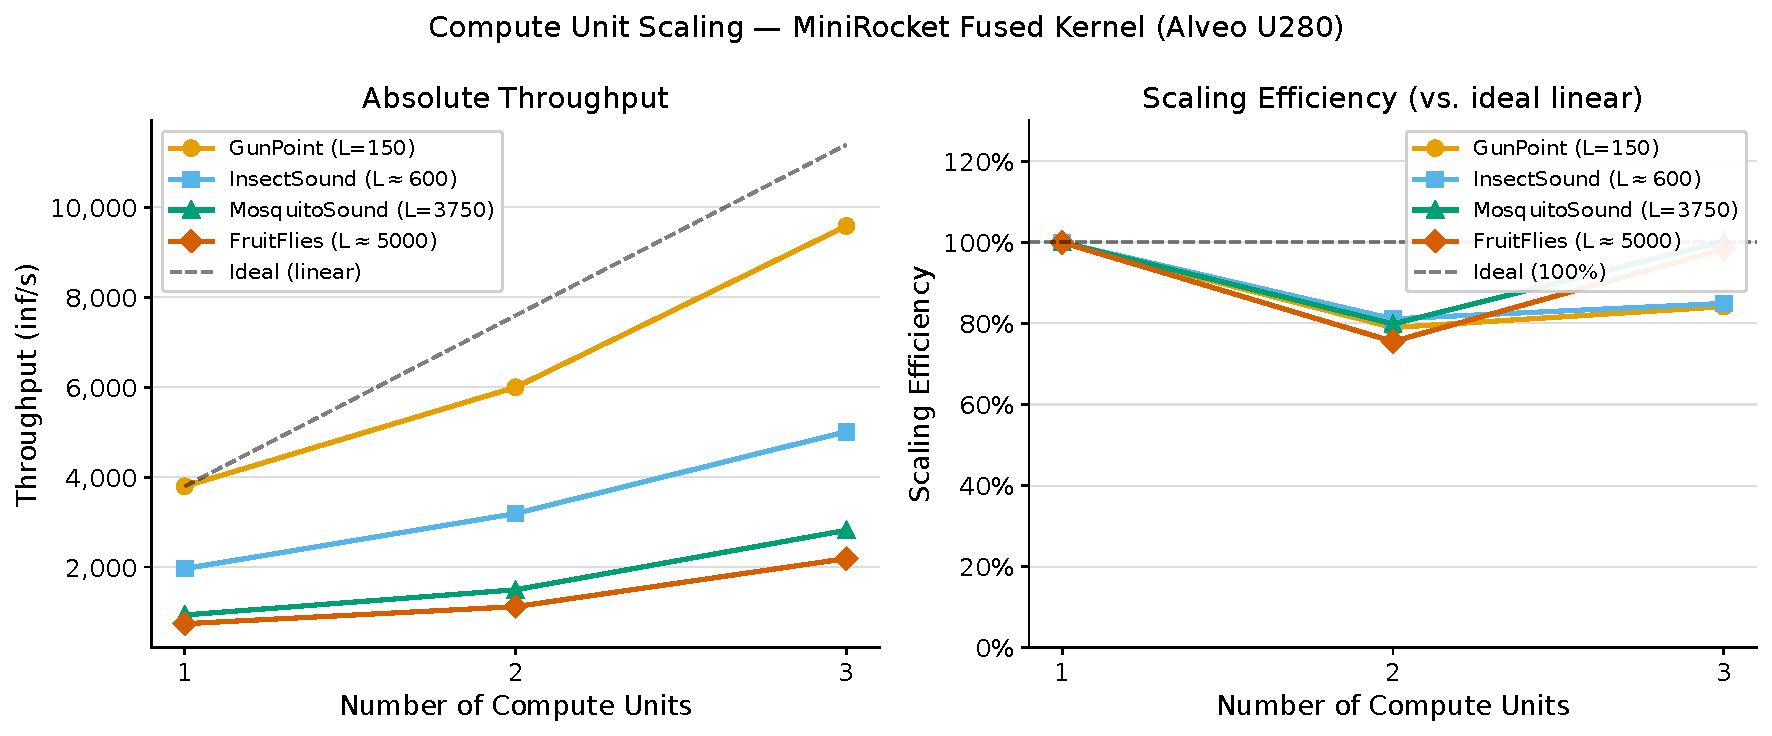
\includegraphics[width=\linewidth]{Figures/fig4_scaling.pdf}
    \caption{MiniRocket GPU/FPGA throughput ratio vs.\ time series length. GPU: Tesla T4, batch=256 and batch=1. FPGA: Alveo U280, fused 1-CU, 300\,MHz.}
    \label{fig:gpu_scalability}
\end{figure}

Fig. \ref{fig:gpu_scalability} shows how the GPU/FPGA throughput ratio varies with time series length. The GPU advantage at batch=256 drops from 65$\times$ at length 64 to 3.8$\times$ at length 8,192. At batch=1, the FPGA matches the GPU at length $\sim$4,096 (single CU) and $\sim$2,048 (3-CU).

Table~\ref{tab:power} compares energy efficiency across platforms. The FPGA consumes 25.7\,W (measured via \texttt{xbutil examine}); the GPU consumes 54--68\,W under sustained inference; CPU power is measured via Intel RAPL at 40--53\,W under single-threaded inference. For long time series (MosquitoSound), the FPGA 3-CU configuration achieves 92$\times$ better energy efficiency than the CPU baseline and 1.4$\times$ better than the GPU at batch=256. For short series (InsectSound), the GPU's higher batched throughput yields 2.3$\times$ better energy efficiency; the FPGA advantage re-emerges at batch=1. Hydra exhibits similar trends: at 25.7\,W, the 3-CU FPGA consumes 2.4--8.6\,mJ/inf across datasets.

\begin{table}[t]
\centering
\caption{Energy efficiency: MiniRocket inference. FPGA 25.7\,W (static-dominated at $<$5\% utilization); GPU via nvidia-smi; CPU via RAPL.}
\label{tab:power}
\resizebox{\columnwidth}{!}{
\begin{tabular}{llrrrr}
\toprule
Dataset & Platform & Tput (inf/s) & Power (W) & mJ/inf & vs CPU \\
\midrule
InsectSound & CPU C++ & 289 & 52.8 & 182.7 & 1$\times$ \\
 & GPU T4 (b=256) & 30,469 & 68 & 2.2 & 83$\times$ \\
 & FPGA 3-CU & 5,012 & 25.7 & 5.1 & 36$\times$ \\
\midrule
MosquitoSound & CPU C++ & 48 & 40.0 & 833.3 & 1$\times$ \\
 & GPU T4 (b=256) & 4,198 & 54 & 12.9 & 65$\times$ \\
 & FPGA 3-CU & 2,820 & 25.7 & 9.1 & 92$\times$ \\
\midrule
FruitFlies & CPU C++ & 258 & 49.9 & 193.4 & 1$\times$ \\
 & GPU T4 (b=256) & 3,227 & 54 & 16.7 & 12$\times$ \\
 & FPGA 3-CU & 2,191 & 25.7 & 11.7 & 17$\times$ \\
\bottomrule
\end{tabular}}
\end{table}


\subsection{Network Streaming Results}
\label{sec:streaming_results}

In the MiniRocket SmartNIC experiment (ArrowHead dataset), the FPGA achieves 4.12\,ms average RTT (1.25\,ms computation + 2.87\,ms communication) vs.\ 11.0\,ms for CPU with Python sockets (2.65$\times$). With DPDK kernel bypass, CPU RTT drops to 5.66\,ms (2.31\,ms computation + 3.35\,ms communication); the FPGA retains a 1.37$\times$ advantage, with gains in both computation (1.85$\times$) and communication (1.17$\times$).

